\documentclass[11pt,a4paper]{article}
\usepackage[T1]{fontenc}
\usepackage{lmodern}
\usepackage[margin=20mm]{geometry}
\usepackage{graphicx}
\usepackage{booktabs}
\usepackage{amsmath}
\usepackage{caption}
\usepackage{pdflscape}
\usepackage[hidelinks]{hyperref}

\graphicspath{{analysis_output/review/figures/}}
\captionsetup{font=small,labelfont=bf}
\setlength{\parindent}{0pt}
\setlength{\parskip}{6pt}

\title{Figures and tables for 4 games across the 5 variants}
\author{}
\date{}

\begin{document}
\maketitle
\vspace{-2em}

The completed experiments cover Breakout, Asterix, Freeway, and Space Invaders,
with five algorithmic variants and 30 matched configuration--seed individuals
per variant and game (600 completed runs). Each run used five million training
frames, with evaluation every 50,000 frames over ten fixed-seed greedy episodes.
Space Invaders extends the three environments specified in the proposal.

\begin{table}[htbp]
    \centering
    \caption{Mean area under the evaluation learning curve (AUC), in
    $10^6$ return $\times$ frames. Parentheses show the percentage change
    relative to Standard DQN within each game.}
    \label{tab:mean-auc}
    \small
    \setlength{\tabcolsep}{4pt}
    \resizebox{\textwidth}{!}{%
    \begin{tabular}{lrrrr}
        \toprule
        Variant & Breakout & Asterix & Freeway & Space Invaders \\
        \midrule
        Standard DQN & 65.21 & 16.77 & 159.81 & 168.84 \\
        Double DQN & 65.31 ($+0.1\%$) & 21.49 ($+28.2\%$) & 146.18 ($-8.5\%$) & 188.03 ($+11.4\%$) \\
        PER & 65.29 ($+0.1\%$) & 14.12 ($-15.8\%$) & 114.11 ($-28.6\%$) & 80.97 ($-52.0\%$) \\
        $n$-step DQN & \textbf{68.13 ($+4.5\%$)} & 3.35 ($-80.0\%$) & 64.86 ($-59.4\%$) & 133.38 ($-21.0\%$) \\
        Averaged DQN & 65.91 ($+1.1\%$) & \textbf{26.41 ($+57.5\%$)} & \textbf{193.21 ($+20.9\%$)} & \textbf{201.72 ($+19.5\%$)} \\
        \bottomrule
    \end{tabular}%
    }
\end{table}

Table~\ref{tab:mean-auc} reports the proposal's primary outcome, averaging
each run's AUC across the 30 individuals. AUC integrates mean evaluation
return over the observed interval from 50,000 to 5,000,000 frames; higher
values indicate greater accumulated evaluation performance during training.
Percentage changes are calculated from the unrounded variant and control
means. Bold entries identify the highest observed mean in each game, not
statistical significance. Averaged DQN has the highest mean in three games,
while $n$-step DQN has the highest mean in Breakout.

\section*{Statistical overview}
The analysis compares each treatment with its matched Standard DQN control
using two-sided paired $t$-tests on individual AUC differences. Following the
proposal, the Bonferroni threshold is $\alpha=0.05/4=0.0125$ for the four
comparisons within each game. The corresponding 98.75\% confidence intervals
are shown in Figure~\ref{fig:paired-effects}.

In Breakout, none of the four comparisons reaches this threshold; the observed
$4.5\%$ advantage of $n$-step DQN is not statistically significant
($p=0.2715$). In Asterix, Averaged DQN has significantly higher mean AUC
($+57.5\%$, $p=0.00170$), and $n$-step DQN has significantly lower mean AUC
($-80.0\%$, $p<0.0001$). Double DQN and PER do not reach the threshold.
In Freeway, Averaged DQN is significantly higher ($+20.9\%$, $p<0.0001$),
while PER and $n$-step DQN are significantly lower ($-28.6\%$ and $-59.4\%$,
respectively; both $p<0.001$). Double DQN's decrease does not reach the
threshold ($p=0.0137$). In Space Invaders, both Double DQN and Averaged DQN
are significantly higher ($+11.4\%$, $p=0.00290$, and $+19.5\%$,
$p<0.0001$), while PER and $n$-step DQN are significantly lower
($-52.0\%$ and $-21.0\%$; both $p<0.001$). These are unadjusted
$p$-values assessed against the per-game threshold.

Shapiro--Wilk tests flag departures from normality in the paired differences
for $n$-step DQN in Breakout, Asterix, and Freeway, and for Double DQN in
Space Invaders ($p<0.05$; Figure~\ref{fig:normality}). The reported
$t$-test results should therefore be read alongside these diagnostics.
Comparisons are against Standard DQN; they do not establish significant
differences between treatments.

\section*{Observations from the figures}
The Breakout learning curves overlap substantially. In Asterix and Freeway,
the Averaged DQN mean curve generally lies above Standard DQN, while
$n$-step DQN remains lower. In Space Invaders, Averaged DQN and Double DQN
generally lie above Standard DQN, and PER remains below it
(Figure~\ref{fig:learning-curves}). The individual AUC plots show substantial
variation within variants, including a broad spread for Averaged DQN in
Asterix and overlapping outcomes in Breakout
(Figures~\ref{fig:auc-distributions} and~\ref{fig:auc-densities}).

The loss plots show different patterns across variants: PER's median logged
loss declines markedly after its initial rise, while several other curves
rise and then level off. In Space Invaders, this decreasing PER loss occurs
alongside a $52.0\%$ lower mean AUC than Standard DQN. Loss magnitude alone
therefore does not describe the observed policy performance; PER also uses
an importance-weighted loss. Loss figures use only available completed logs
matched to saved results, whereas all AUC summaries use the full 30 runs per
variant. Missing loss histories affect Averaged DQN in Breakout and Freeway
and PER in Asterix.

\begin{figure}[htbp]
    \centering
    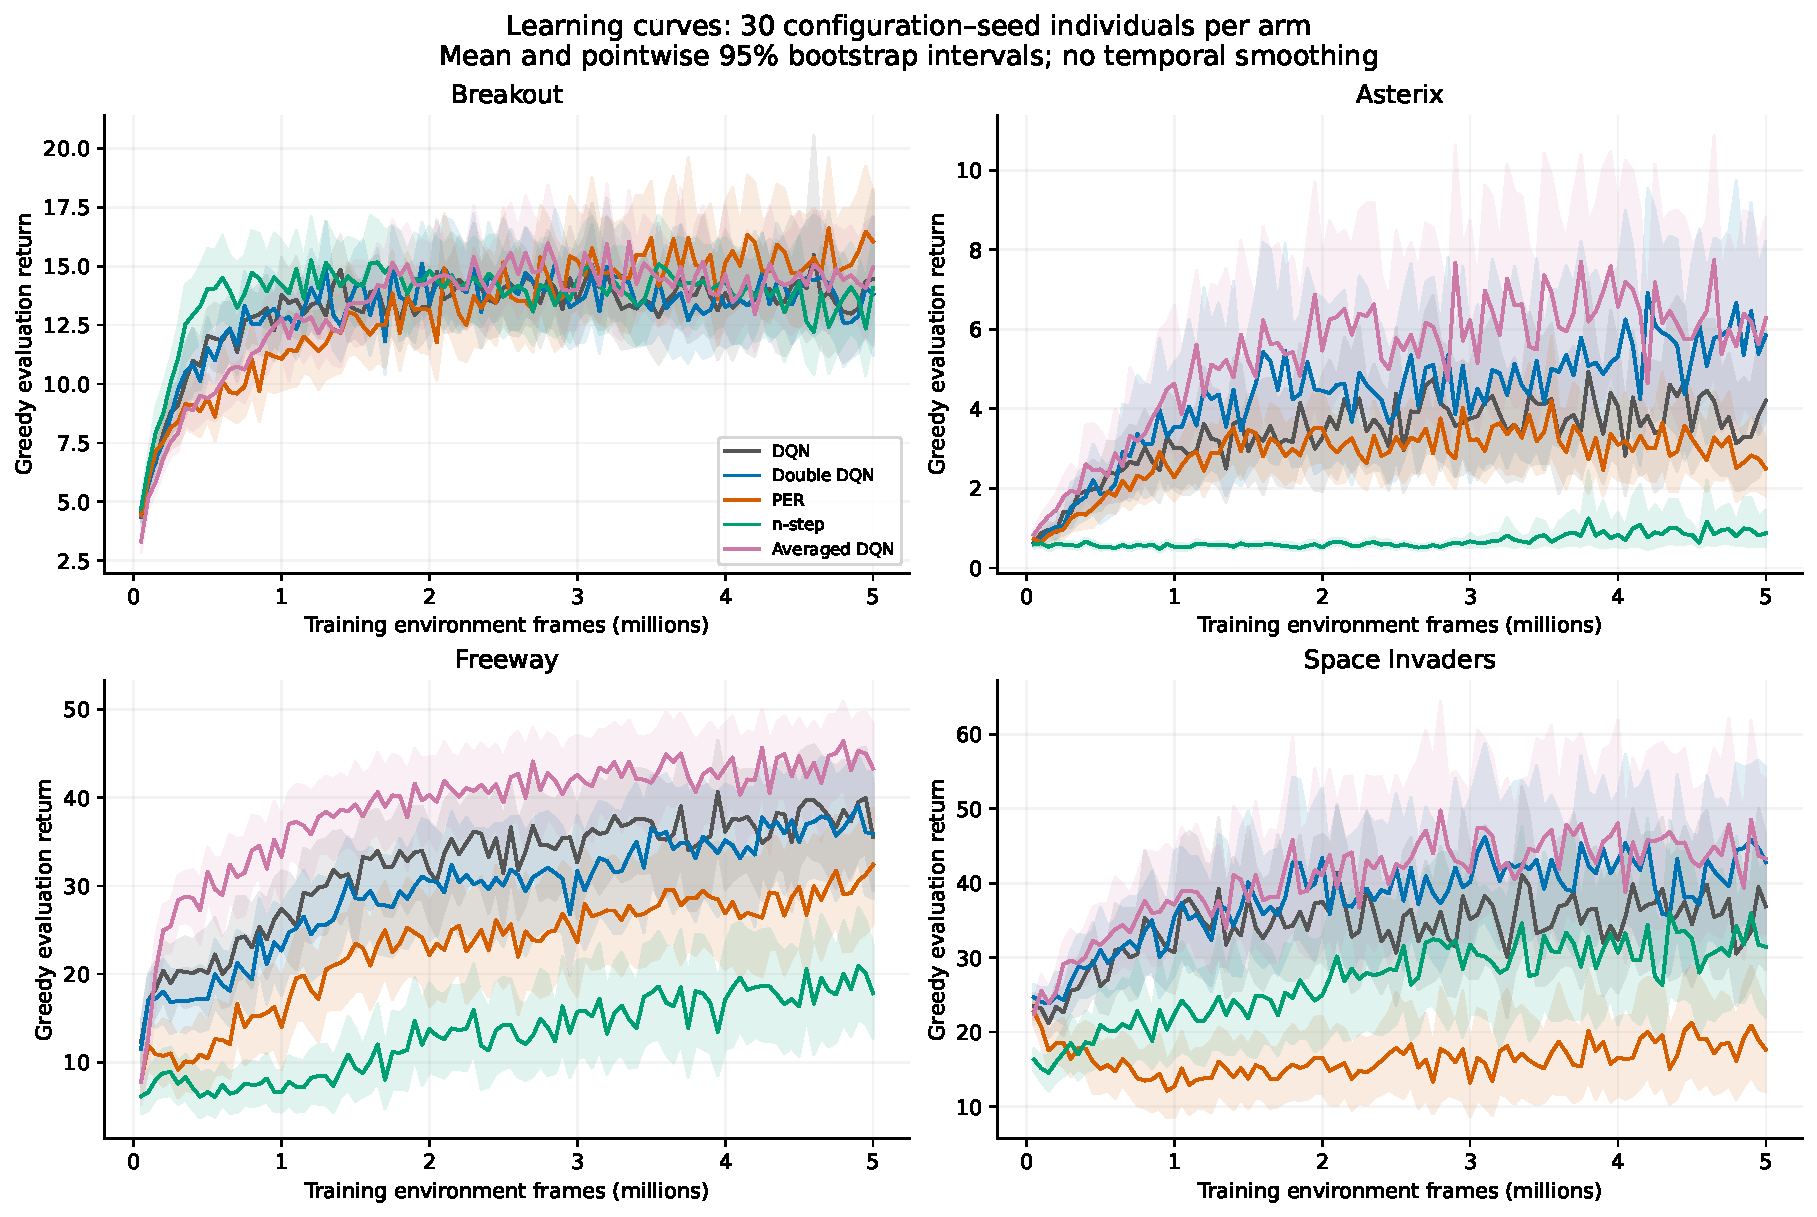
\includegraphics[width=\textwidth]{learning_curves.pdf}
    \caption{Mean greedy evaluation return throughout training for the four
    completed games. Shading shows pointwise 95\% bootstrap confidence
    intervals, resampling whole individuals. Curves are not temporally smoothed.}
    \label{fig:learning-curves}
\end{figure}

\begin{figure}[p]
    \centering
    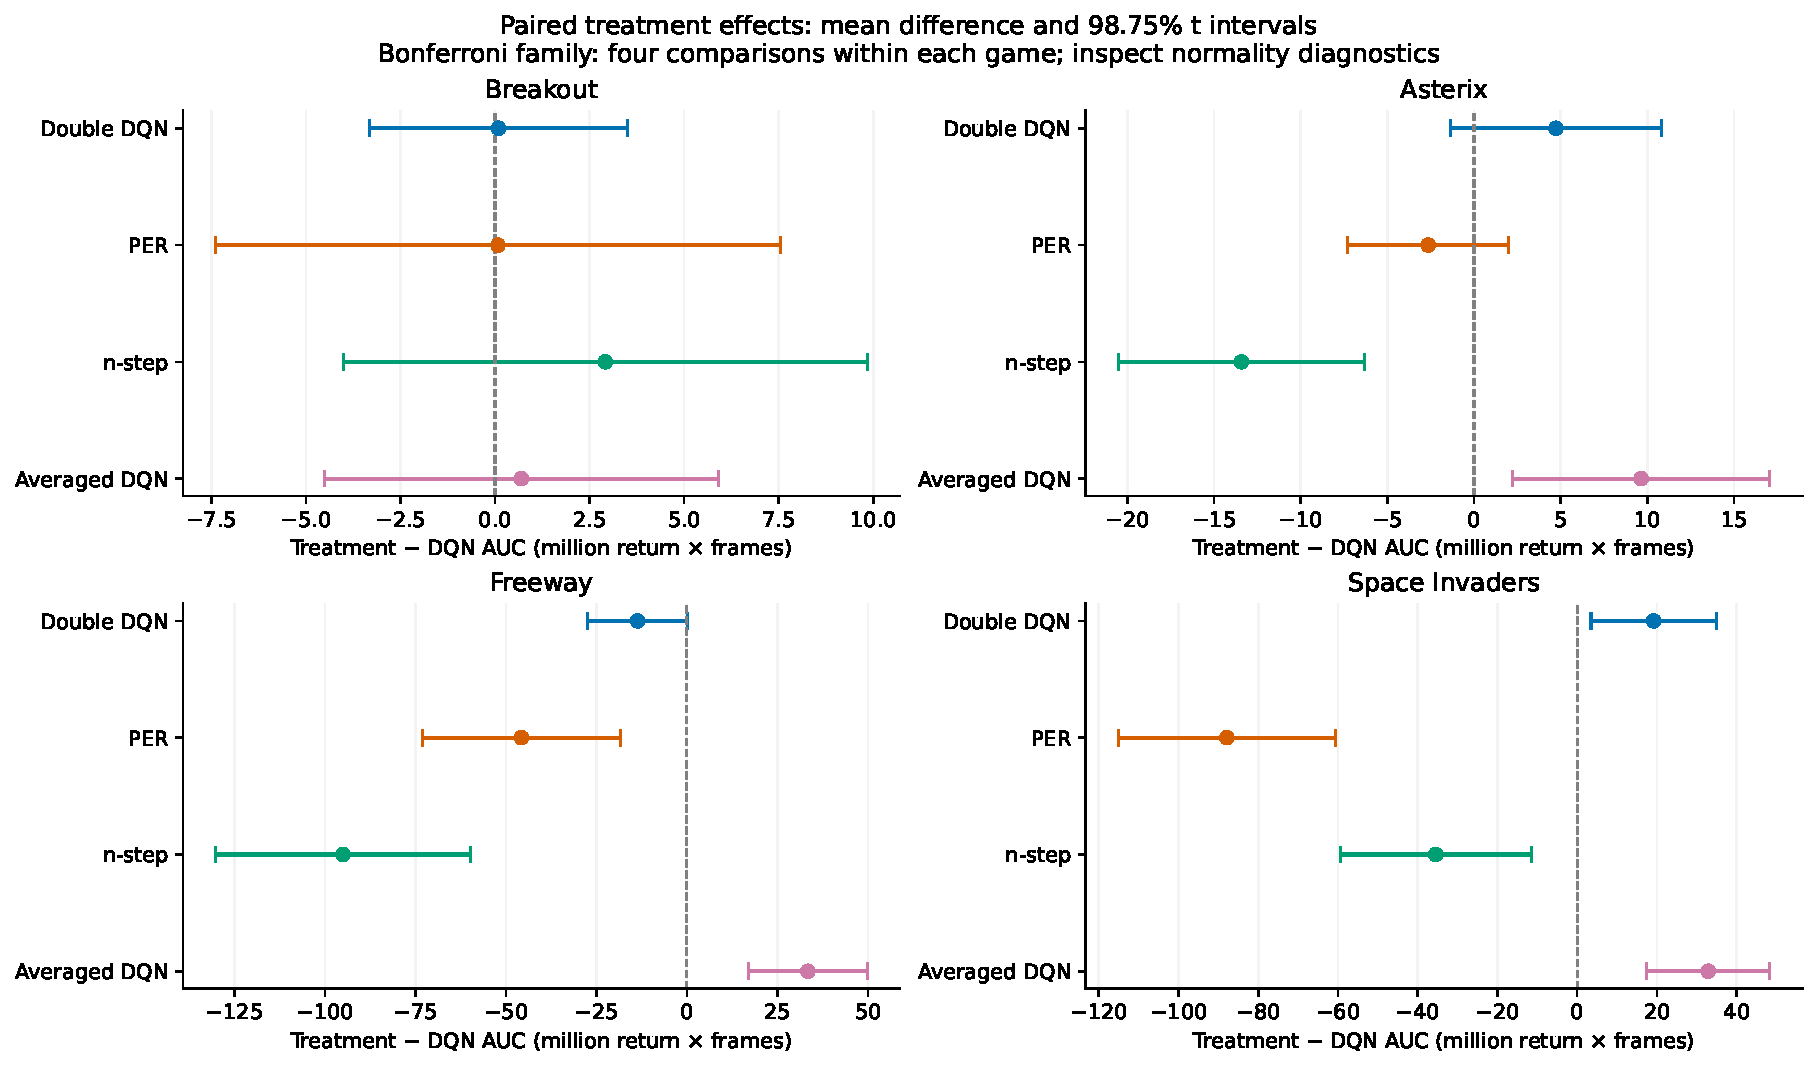
\includegraphics[width=\textwidth]{paired_auc_effects.pdf}
    \caption{Mean paired AUC differences between each treatment and Standard
    DQN, with 98.75\% $t$ confidence intervals. Positive differences favour
    the treatment. Intervals correspond to four treatment--control comparisons
    within each game; all Breakout intervals include zero.}
    \label{fig:paired-effects}
\end{figure}

\begin{figure}[p]
    \centering
    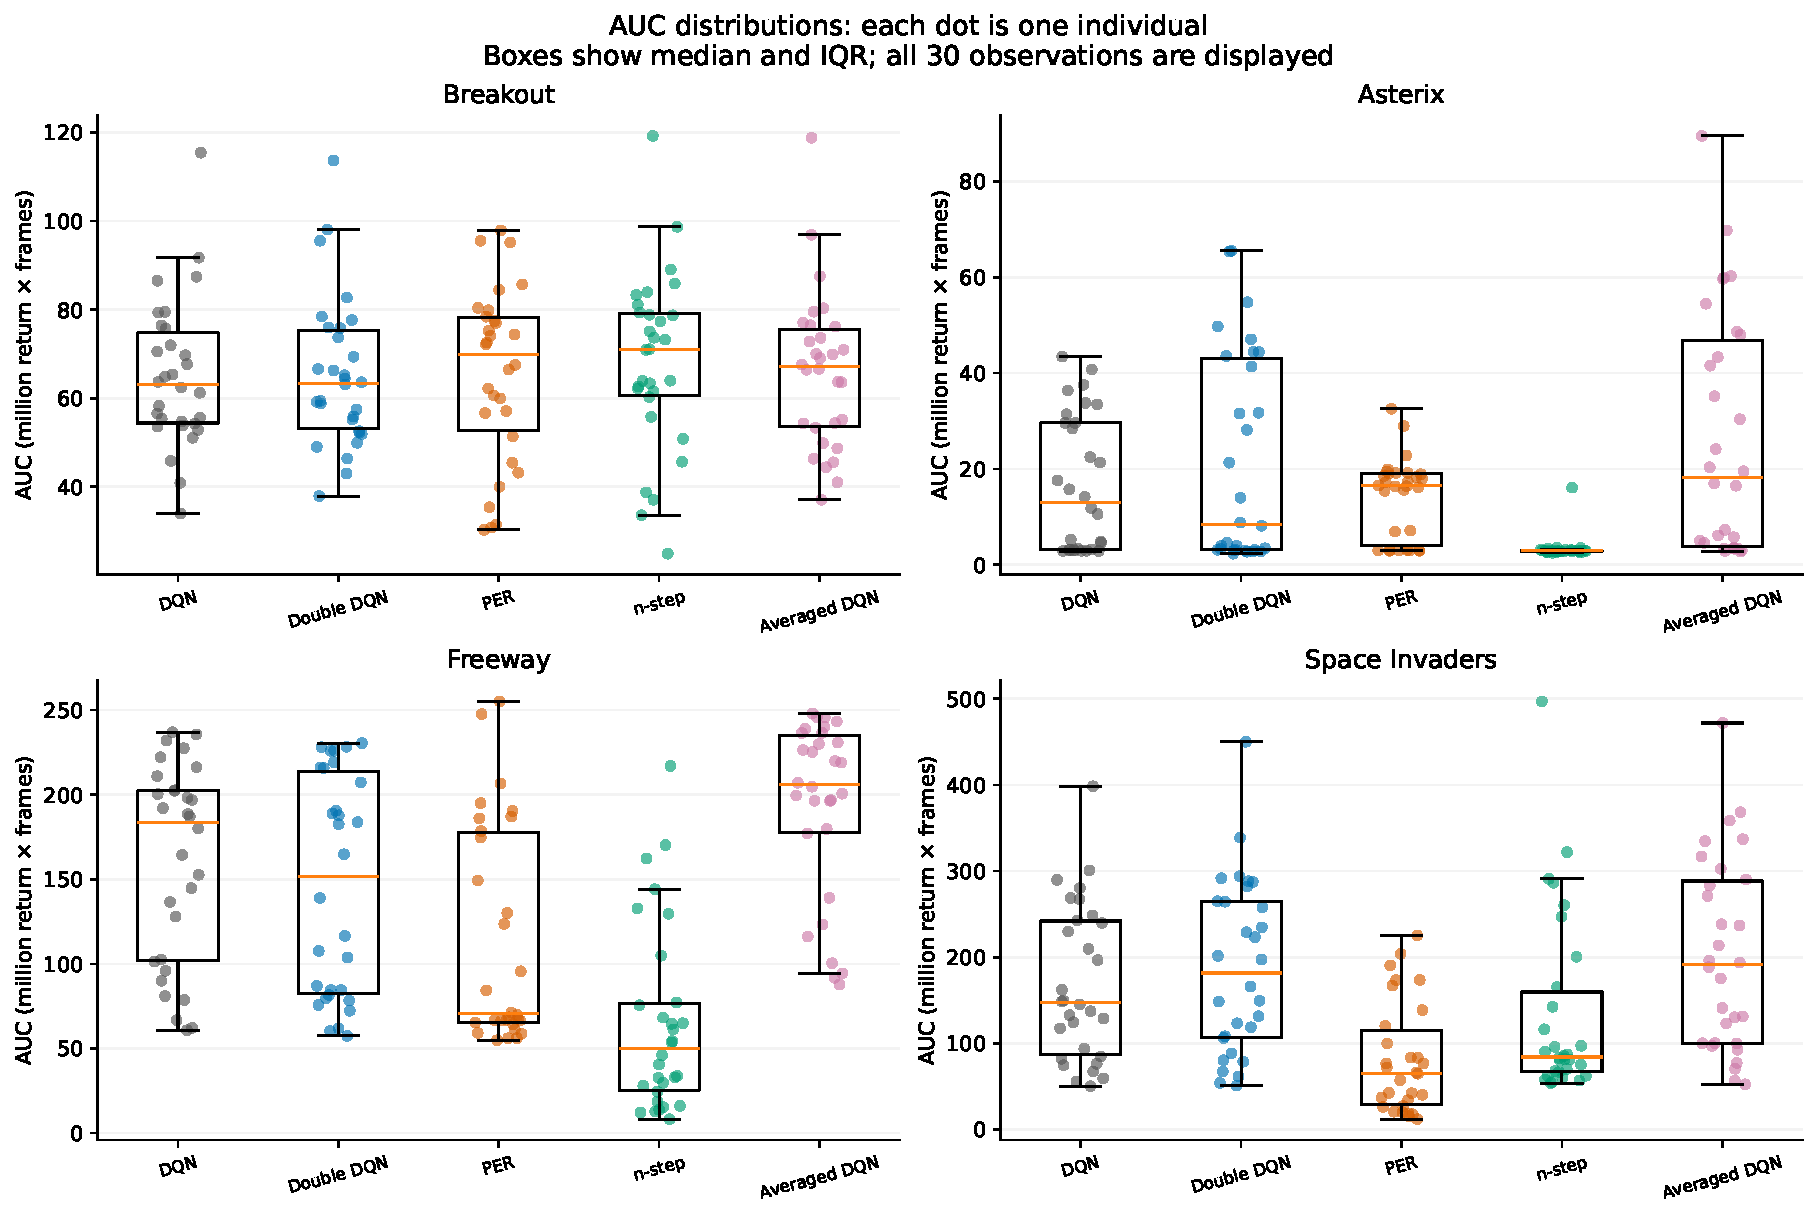
\includegraphics[width=\textwidth]{auc_distributions.pdf}
    \caption{Individual AUC values for each variant and game. Each dot
    represents one completed run; boxes show medians and interquartile ranges.
    All 30 observations per variant are displayed.}
    \label{fig:auc-distributions}
\end{figure}

\begin{figure}[p]
    \centering
    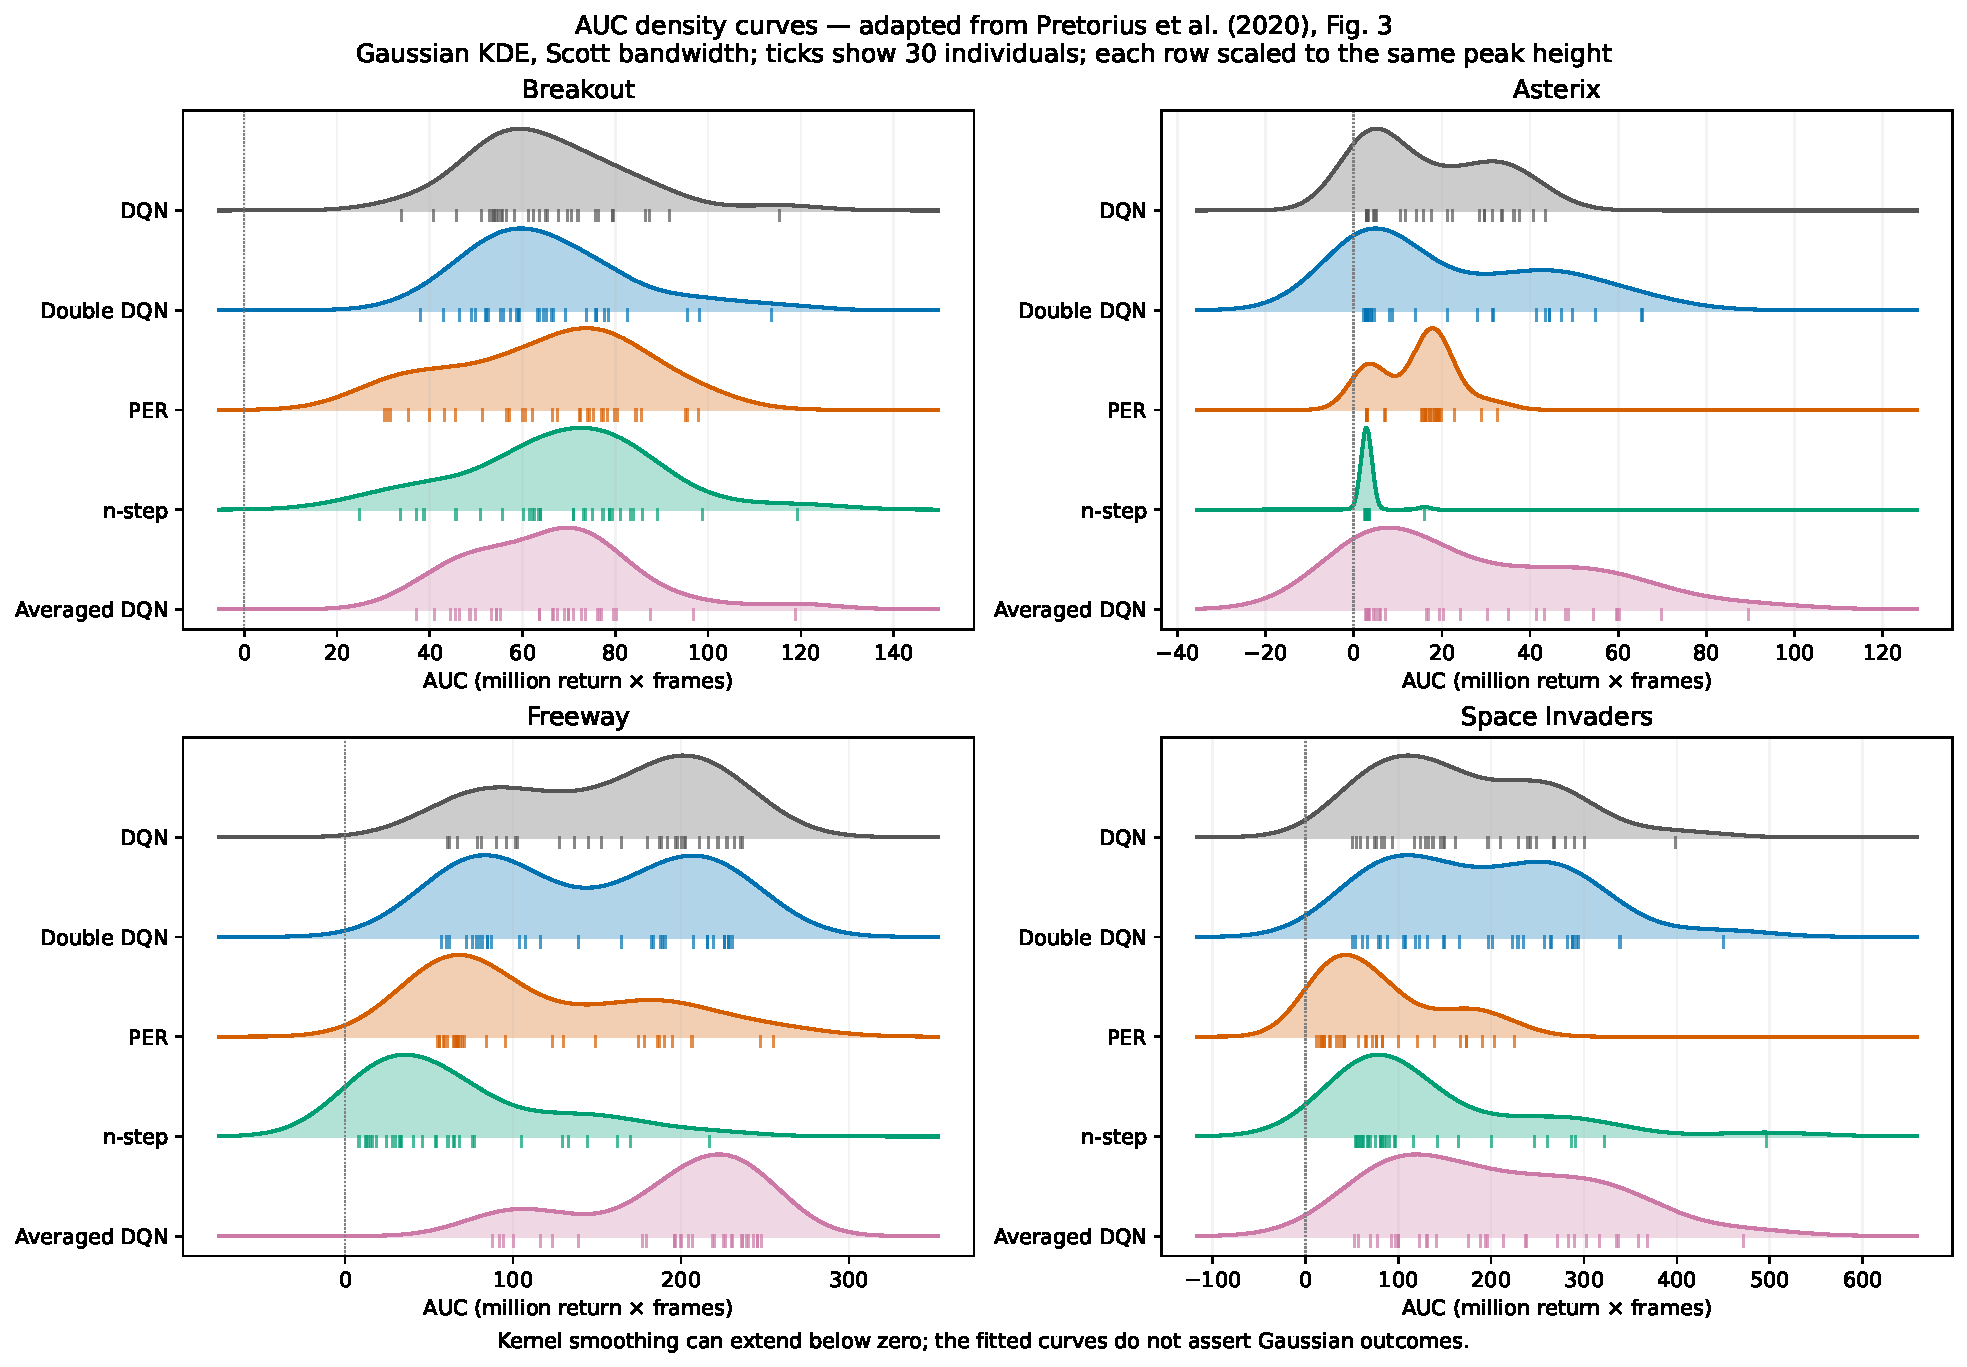
\includegraphics[width=\textwidth]{pretorius_auc_densities.pdf}
    \caption{Smoothed AUC distributions with individual observations shown
    as ticks. Gaussian kernel density estimates use Scott bandwidth and are
    scaled to the same peak height, so vertical heights cannot be compared
    as probability densities. Smoothing below zero does not represent
    negative observed AUCs.}
    \label{fig:auc-densities}
\end{figure}

\clearpage
\begin{landscape}
\begin{figure}[p]
    \centering
    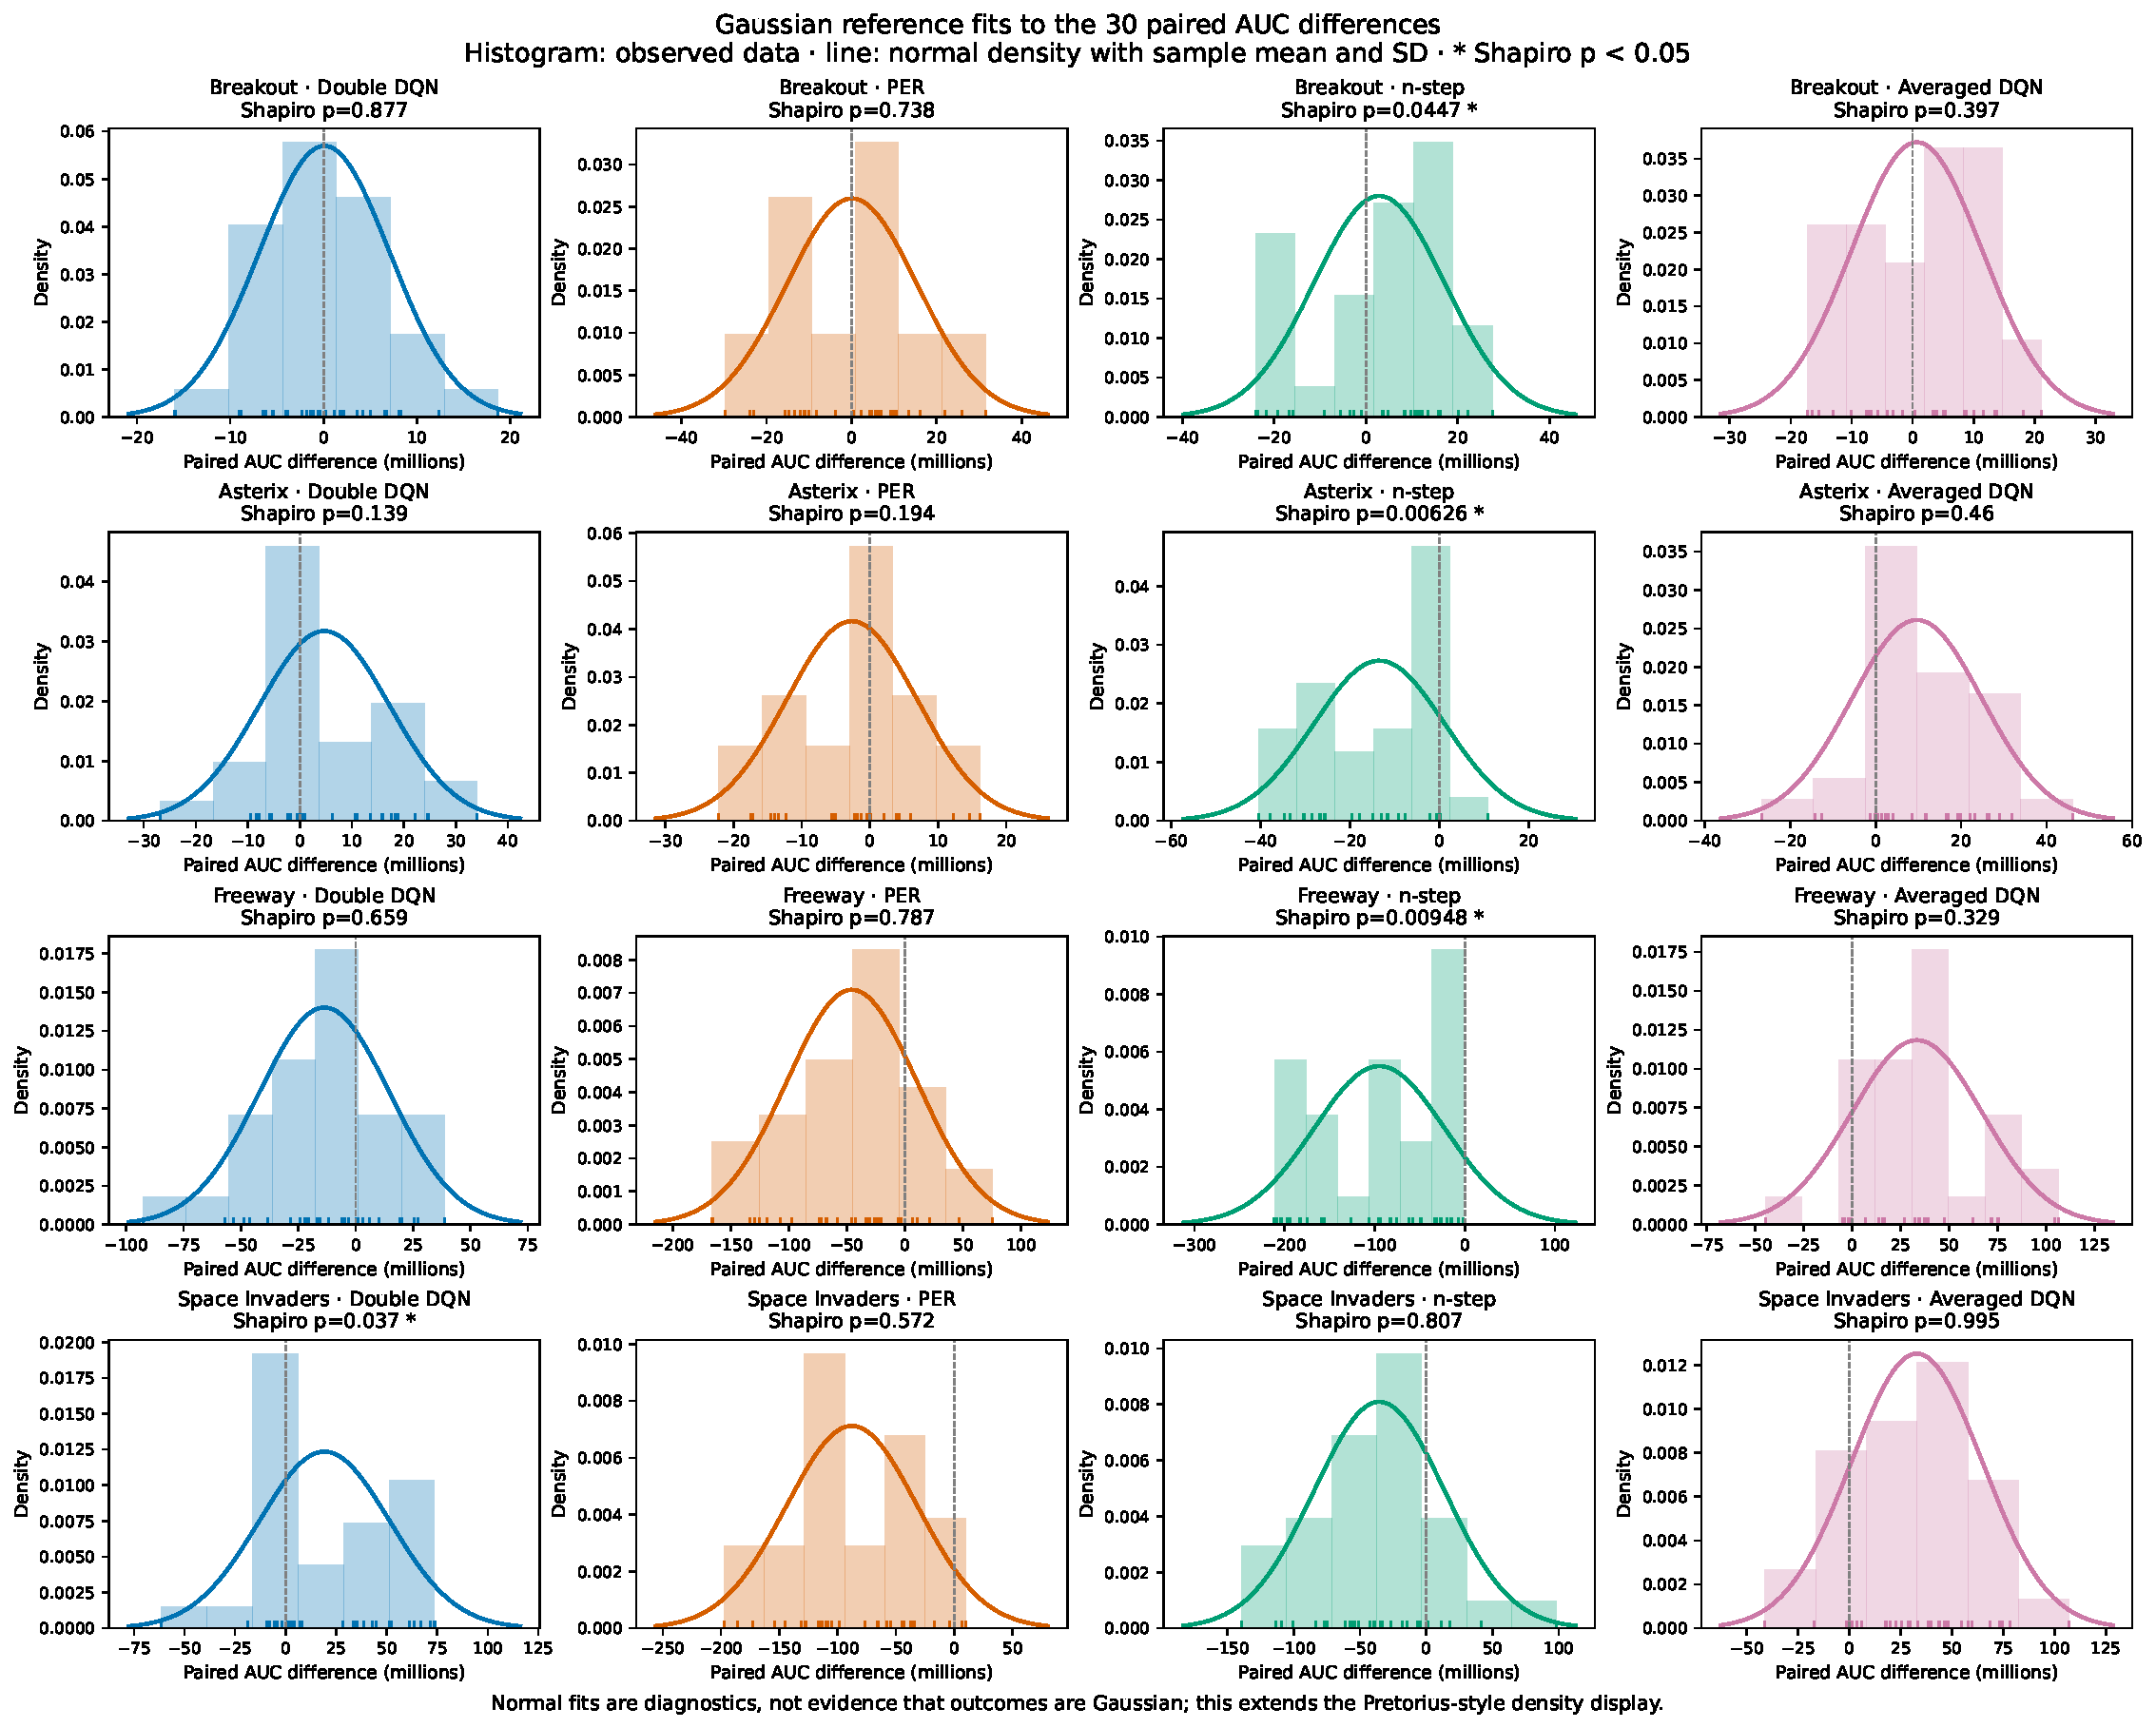
\includegraphics[width=\linewidth,height=0.88\textheight,keepaspectratio]{paired_auc_gaussian_diagnostics.pdf}
    \caption{Distributions of the 30 paired AUC differences for every
    treatment--control comparison. Histograms show observations and lines
    show fitted normal reference densities. Asterisks identify
    Shapiro--Wilk $p<0.05$; the fitted curves are diagnostic references.}
    \label{fig:normality}
\end{figure}
\end{landscape}

\begin{figure}[p]
    \centering
    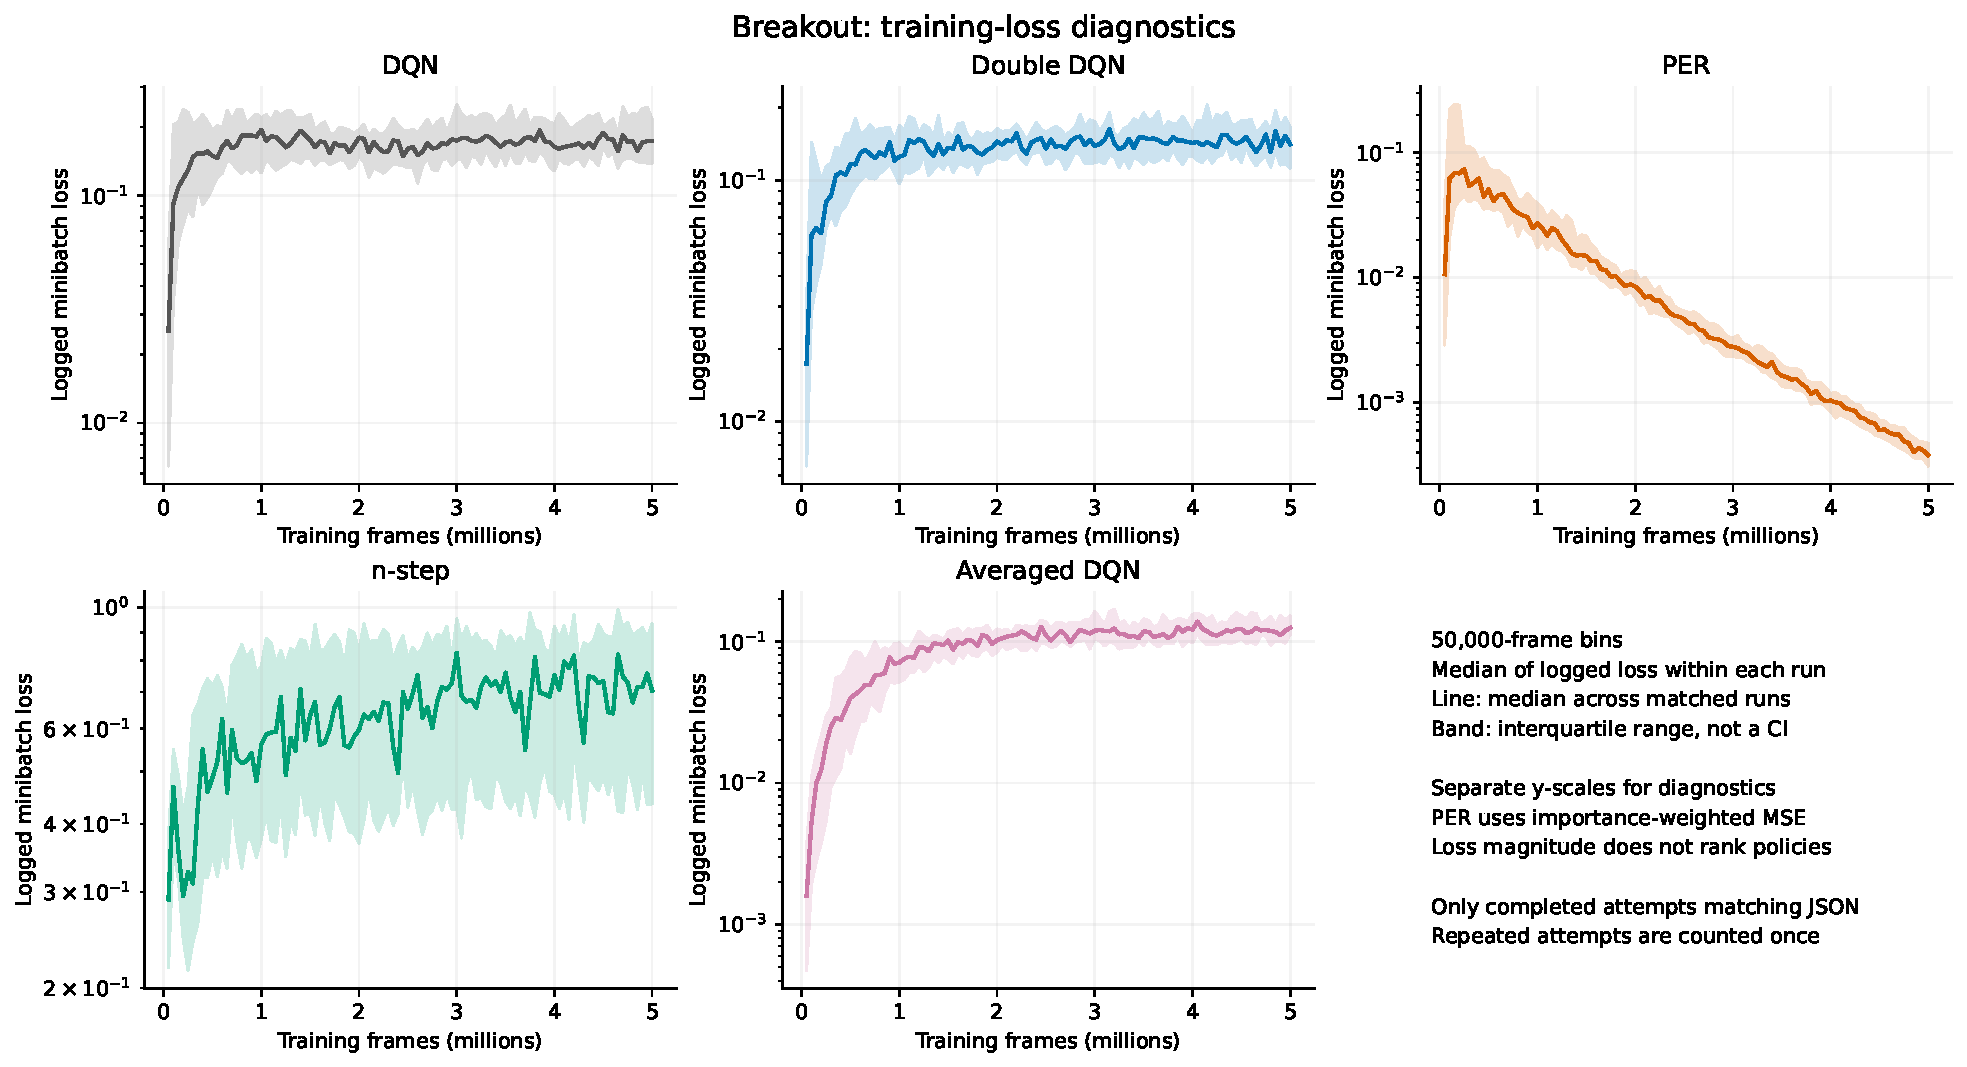
\includegraphics[width=\textwidth]{breakout_loss.pdf}
    \caption{Breakout training losses. Lines show the median across matched
    runs of within-run median loss in 50,000-frame bins; bands show the
    interquartile range, not confidence intervals. Panels use separate
    logarithmic scales. The same conventions apply to the following loss figures.}
    \label{fig:breakout-loss}
\end{figure}

\begin{figure}[p]
    \centering
    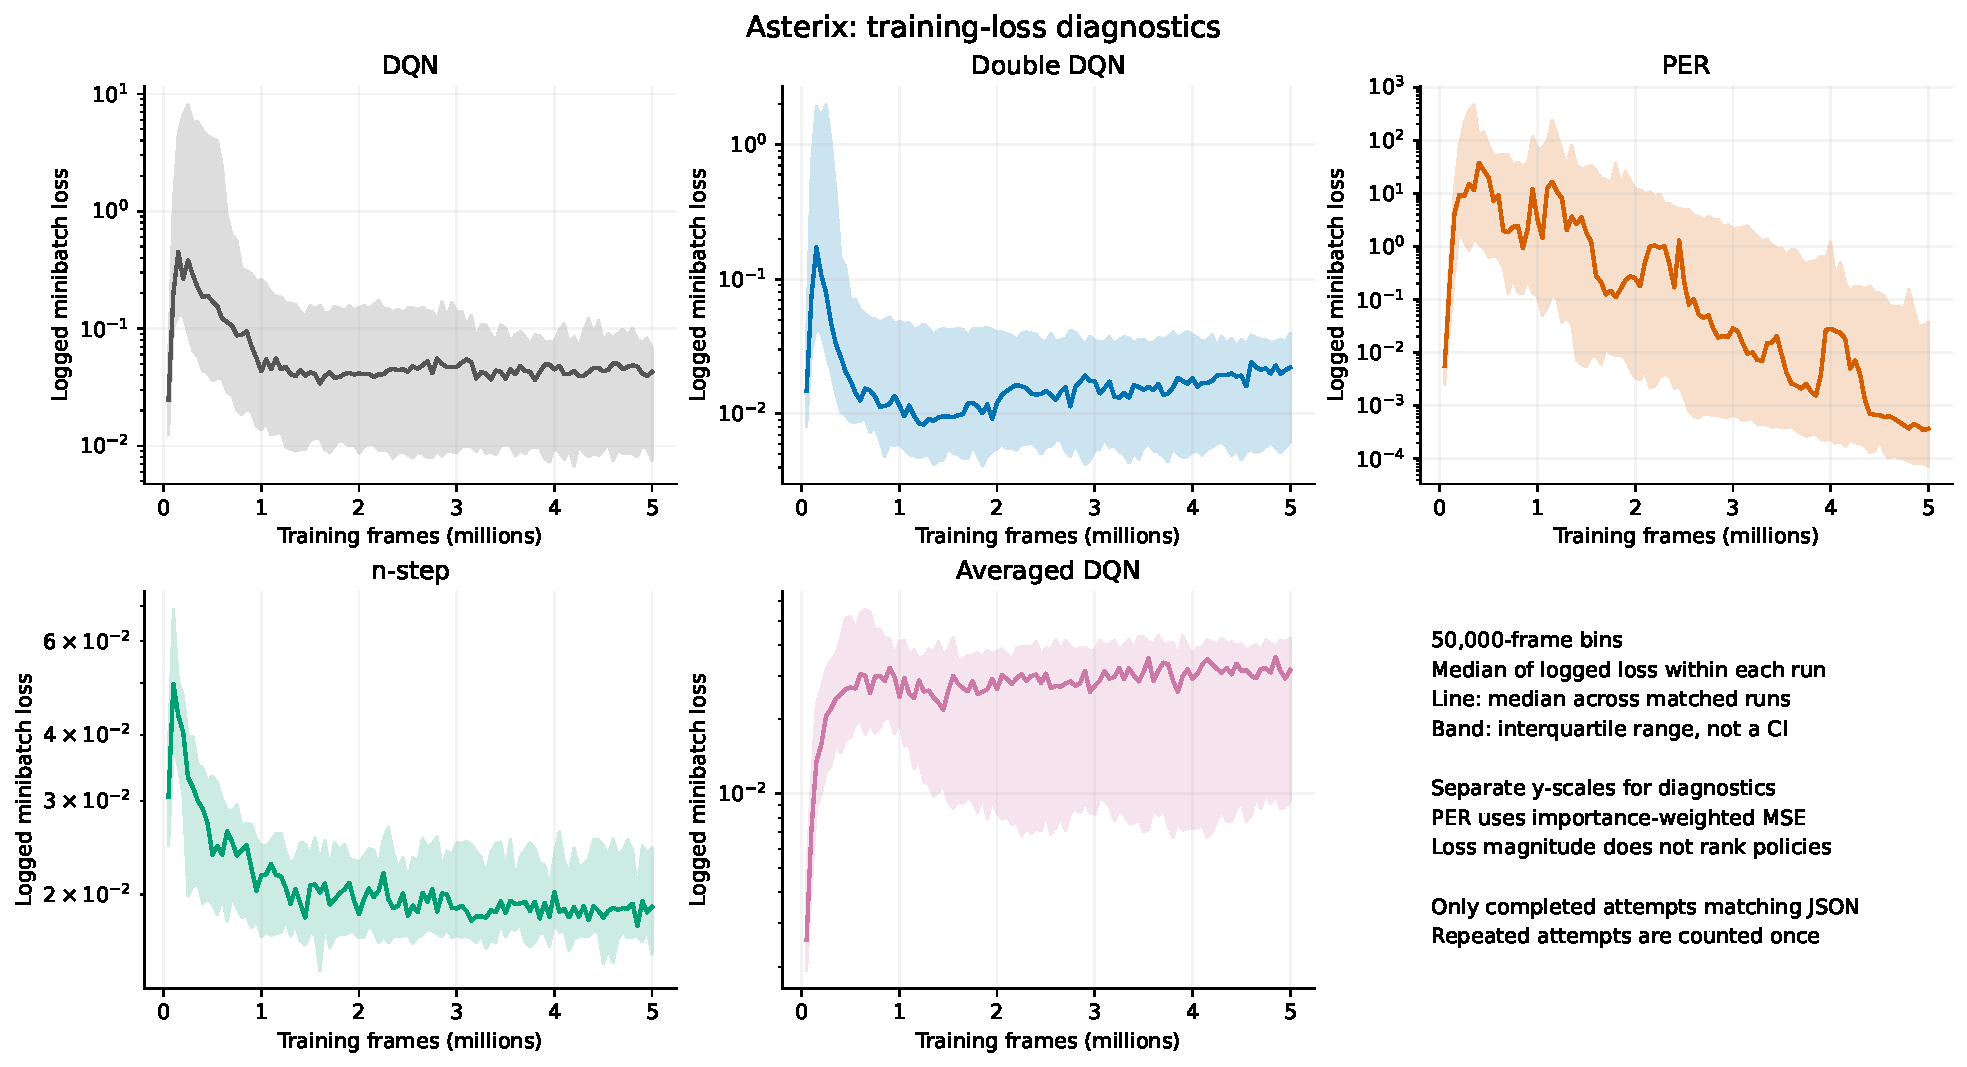
\includegraphics[width=\textwidth]{asterix_loss.pdf}
    \caption{Asterix training losses. PER shows a large early rise followed
    by an uneven decline, while the $n$-step median falls after its early peak.}
    \label{fig:asterix-loss}
\end{figure}

\begin{figure}[p]
    \centering
    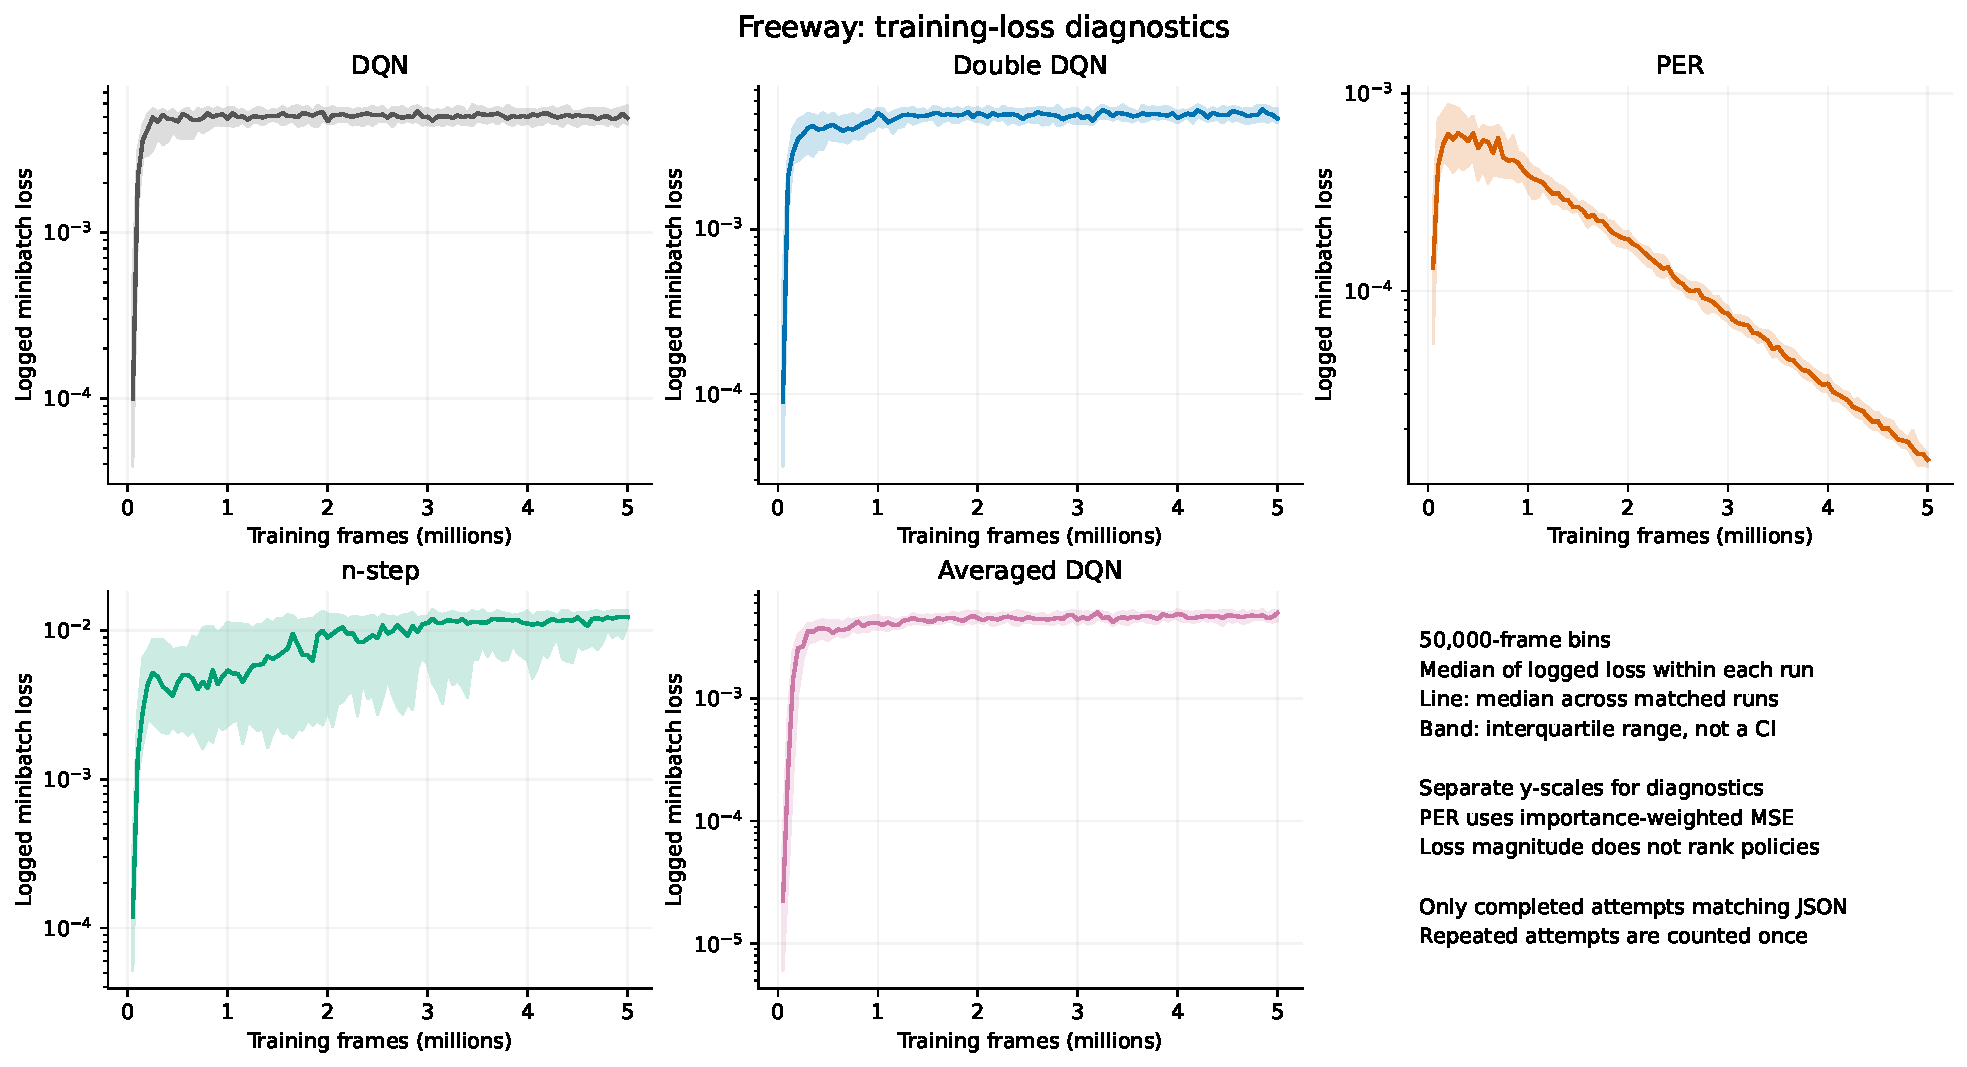
\includegraphics[width=\textwidth]{freeway_loss.pdf}
    \caption{Freeway training losses. Standard DQN, Double DQN, and Averaged
    DQN rise early and then remain comparatively flat. PER's median loss
    declines after its initial rise.}
    \label{fig:freeway-loss}
\end{figure}

\begin{figure}[p]
    \centering
    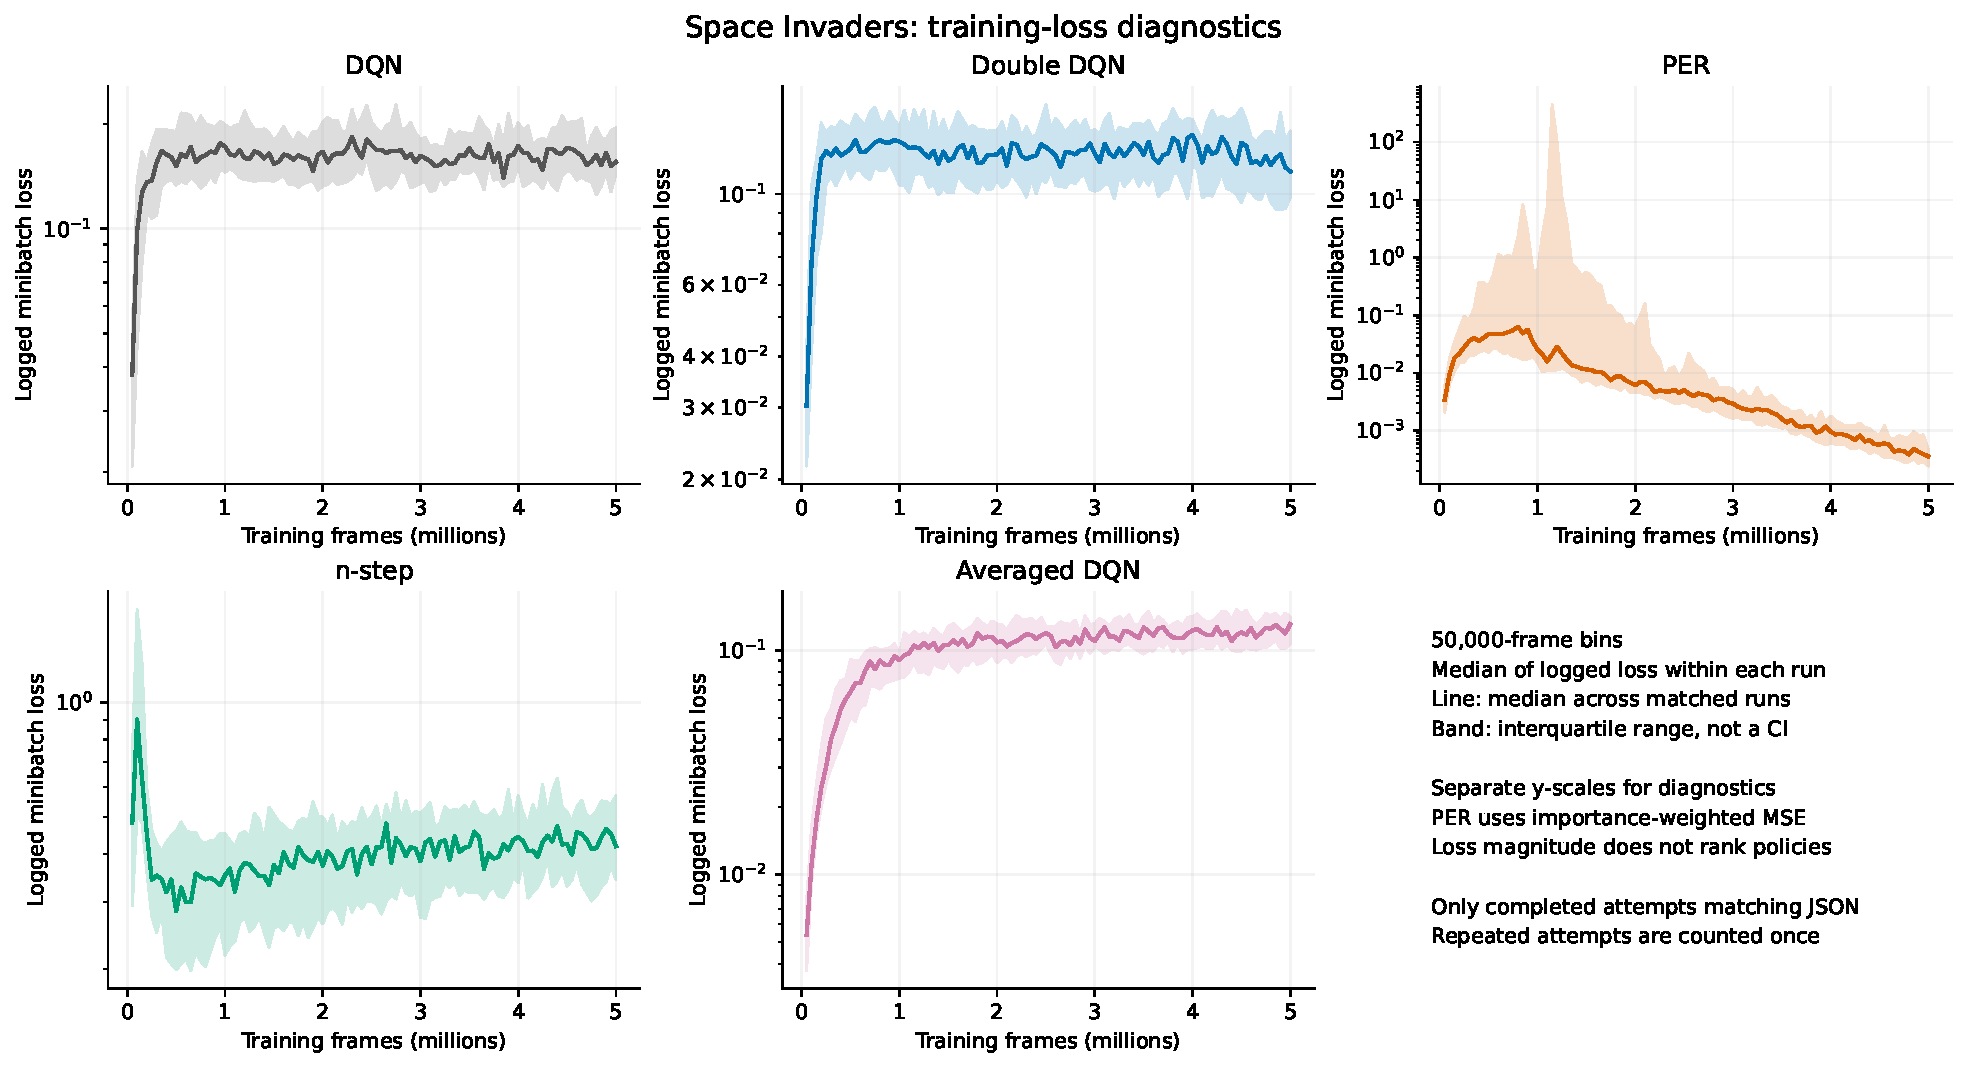
\includegraphics[width=\textwidth]{spaceinvaders_loss.pdf}
    \caption{Space Invaders training losses. PER's median loss decreases
    substantially, although its mean evaluation AUC is below Standard DQN.
    This loss trend does not imply better evaluation performance.}
    \label{fig:spaceinvaders-loss}
\end{figure}

\end{document}
